% Introduction Section
% This file contains the introduction and motivation

\section{Introduction}
\label{sec:introduction}

\begin{figure}[t]
    \centering
    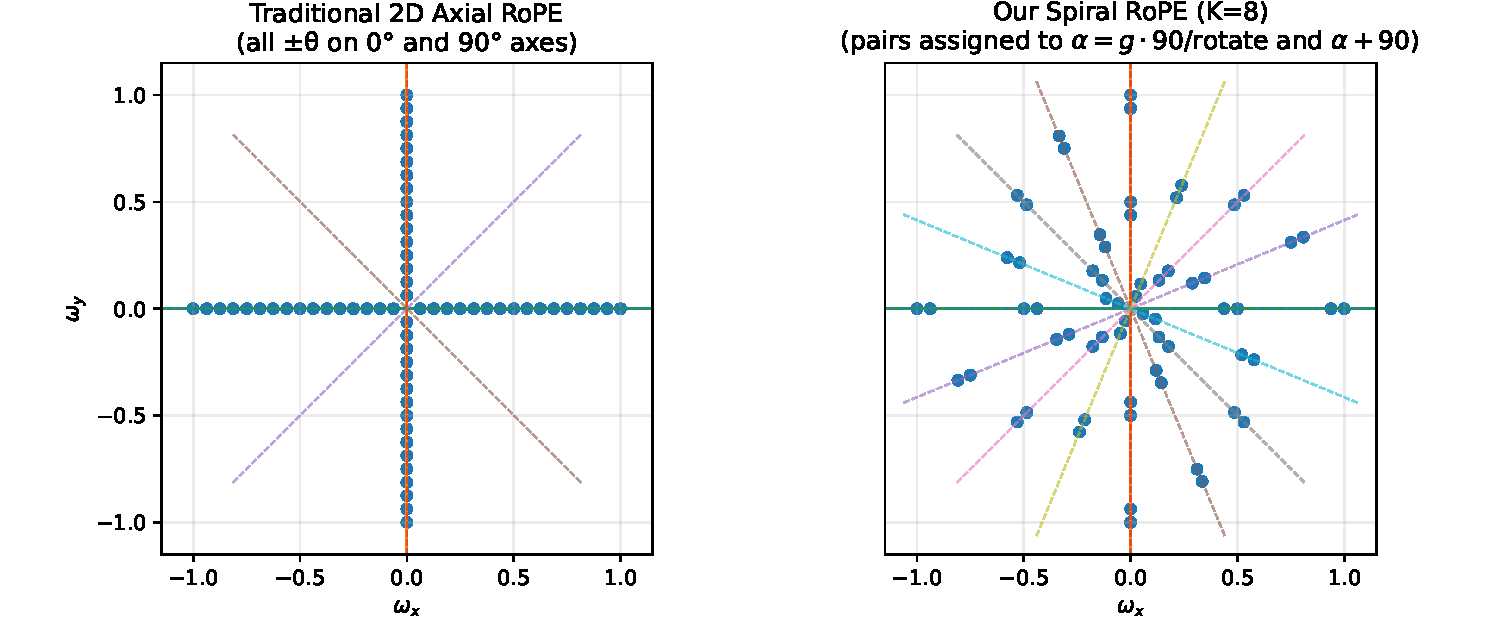
\includegraphics[width=\columnwidth]{plots/rope_K8.pdf}
    \caption{\textbf{\textit{Frequency support visualization}} comparing Axial 2D RoPE \textit{(left)} and Spiral RoPE \textit{(right)} with eight rotation groups ($K=8$). As shown, the Axial 2D RoPE places all frequencies on horizontal and vertical axes only, while our Spiral RoPE distributes frequencies across multiple directions in a spiral pattern, offering a broader directional coverage.}
    \label{fig:teaser}
    \vspace{-0.5cm}
\end{figure}

\begin{figure}[t]
    \centering
    \begin{subfigure}[b]{0.9\columnwidth}
        \centering
        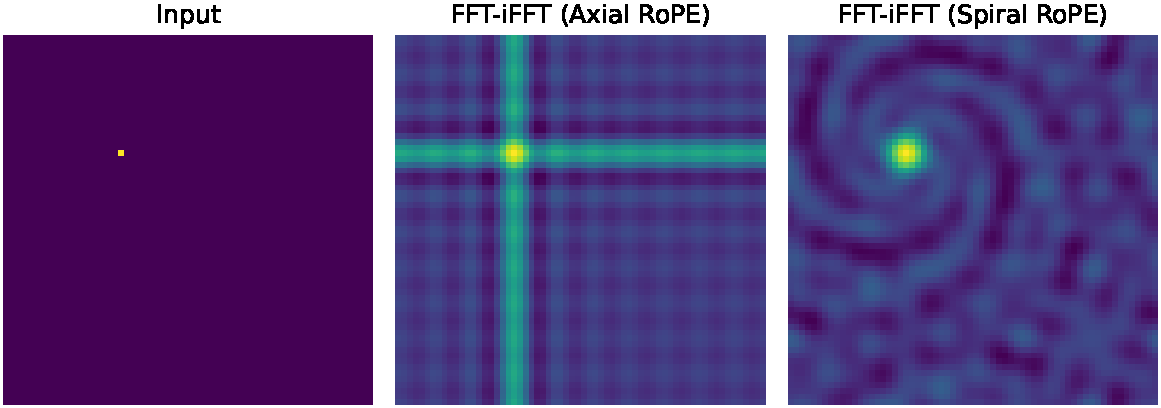
\includegraphics[width=\linewidth]{plots/single.pdf}
        \caption{FFT-iFFT reconstruction of a single point}
    \end{subfigure}
    \hfill
    \begin{subfigure}[b]{0.9\columnwidth}
        \centering
        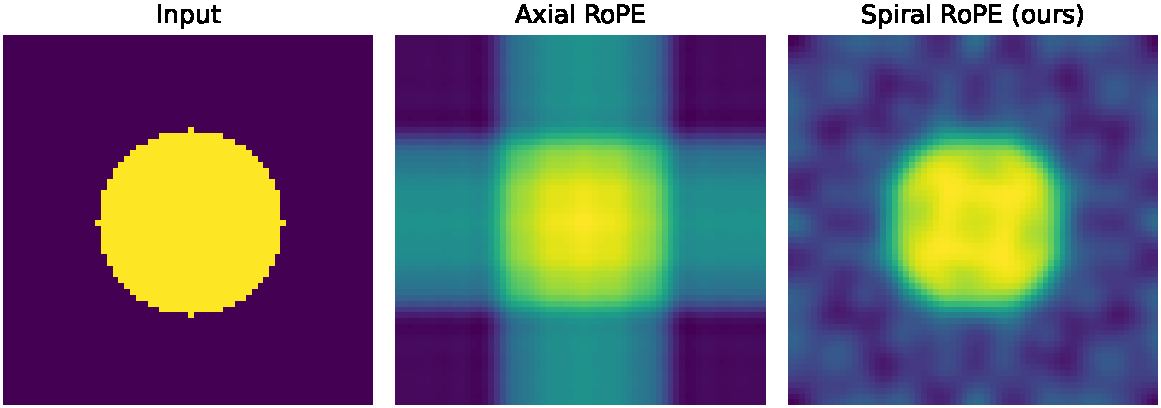
\includegraphics[width=\linewidth]{plots/circle.pdf}
        \caption{FFT-iFFT reconstruction of a circle}
    \end{subfigure}
    \caption{\textbf{\textit{Fourier reconstruction comparisons.}} Given binary input images \textit{(left)}, we retain only frequencies representable by each RoPE method and reconstruct via inverse-FFT. Axial 2D RoPE \textit{(middle)} produces artifacts along horizontal and vertical axes. Spiral RoPE achieves more faithful reconstruction due to broader directional coverage.}
    \vspace{-0.5cm}
    \label{fig:fourier}
\end{figure}

\begin{figure}[t]
    \centering
    \begin{subfigure}[b]{0.9\columnwidth}
        \centering
        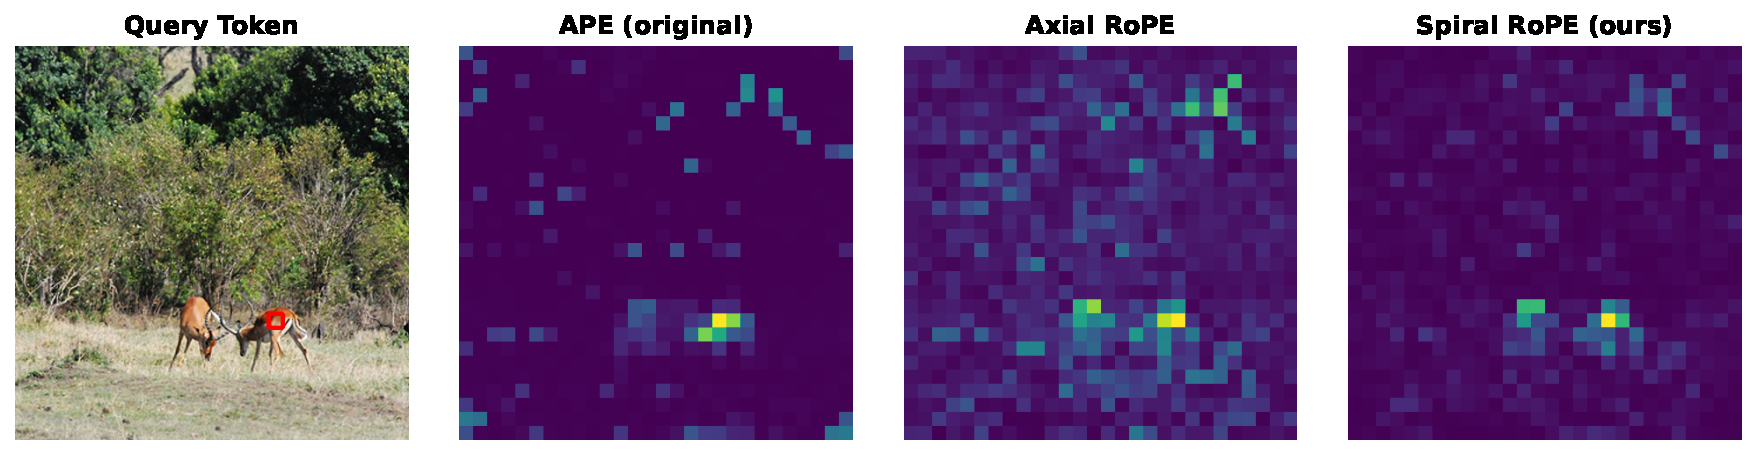
\includegraphics[width=\linewidth]{plots/ILSVRC2012_val_00029872_res448_query_r19_c18_comparison_3models.pdf}
    \end{subfigure}
    \\[0.6em]

    \begin{subfigure}[b]{0.9\columnwidth}
        \centering
        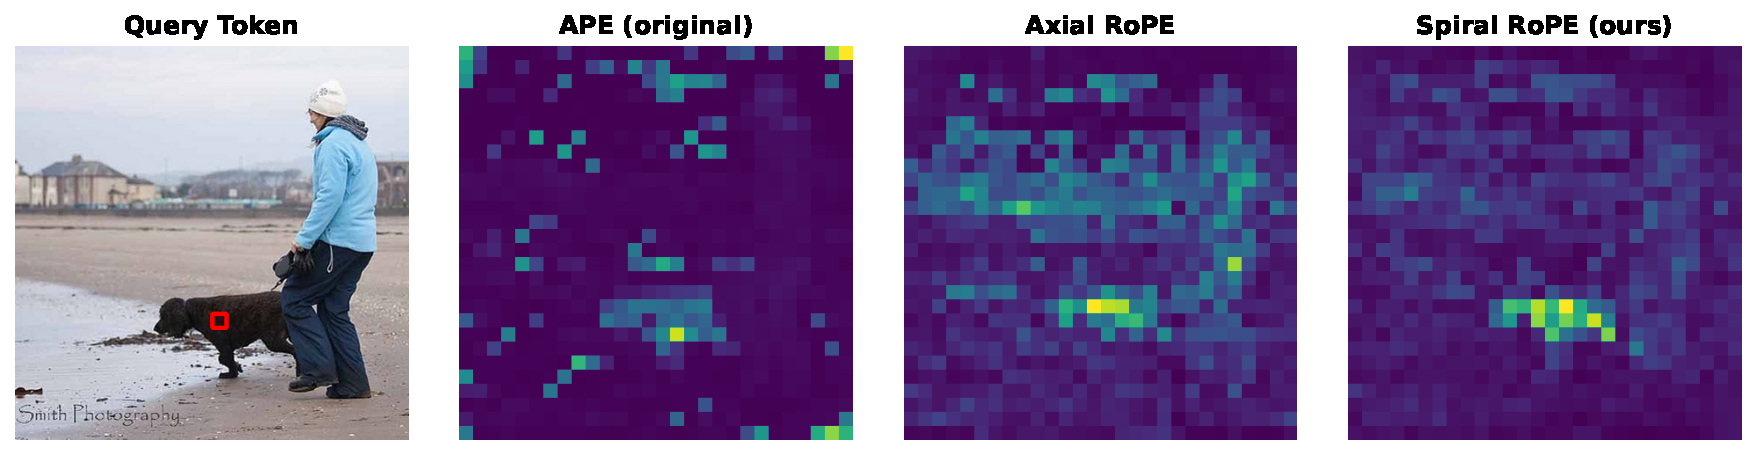
\includegraphics[width=\linewidth]{plots/ILSVRC2012_val_00030920_res448_query_r19_c14_comparison_3models.pdf}
    \end{subfigure}
    \\[0.6em]

    \begin{subfigure}[b]{0.9\columnwidth}
        \centering
        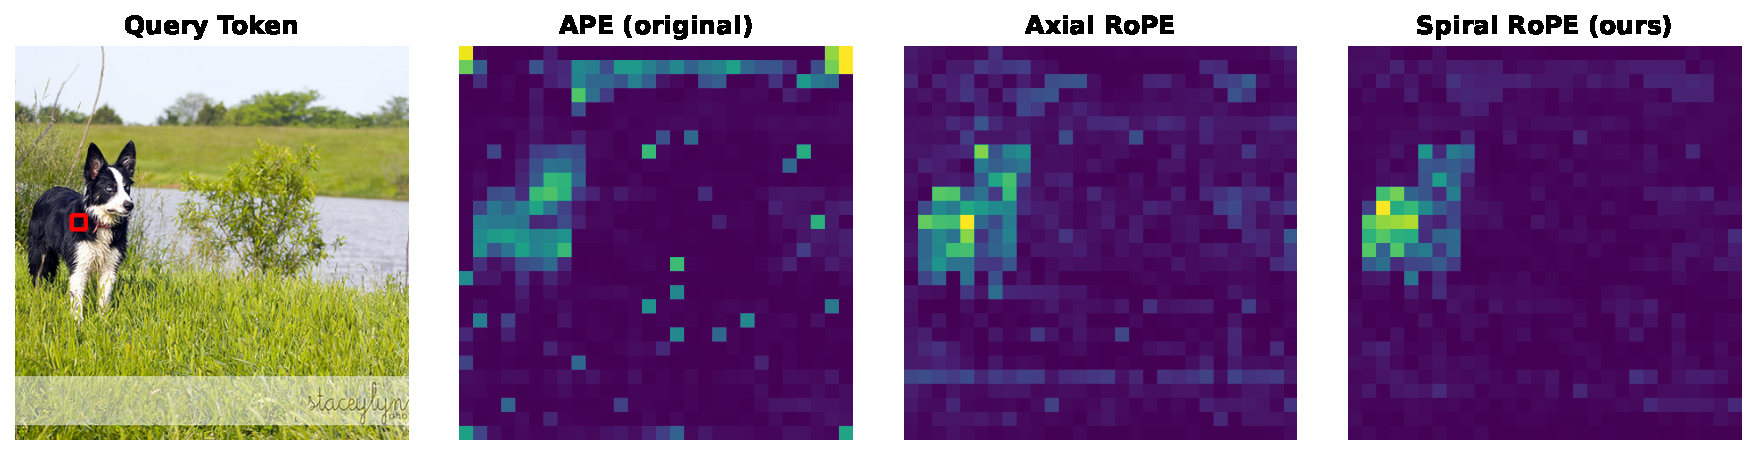
\includegraphics[width=\linewidth]{plots/ILSVRC2012_val_00046446_res448_query_r12_c4_comparison_3models.pdf}
    \end{subfigure}
    \caption{\textbf{\textit{Query-token attention visualization.}} The query token (marked by a red box) is located on a foreground object. Across diverse scenes, Spiral RoPE consistently produces sharper and more localized attention around the queried region compared to APE and Axial RoPE, indicating improved spatial alignment.}
    \label{fig:query_attn}
\end{figure}


Rotary Position Embedding (RoPE)~\cite{suRoFormerEnhancedTransformer2023} has become a cornerstone of modern language transformers, powering state-of-the-art large language models such as the LLaMA series~\cite{touvronLLaMAOpenEfficient2023, touvronLlama2Open2023, grattafioriLlama3Herd2024} and Qwen series~\cite{baiQwenTechnicalReport2023, yangQwen2TechnicalReport2024, yangQwen25TechnicalReport2025, yangQwen3TechnicalReport2025}. By encoding positional information through rotation operations on query and key vectors, RoPE naturally captures relative positions and enables effective length extrapolation. Such properties have been proven essential for scaling transformers to long contexts. In contrast, standard Vision Transformers (ViTs)~\cite{dosovitskiyImageWorth16x162021} predominantly rely on absolute positional embeddings (APE), which encode fixed position vectors that are added to patch embeddings. While simple and effective, APE has well-documented limitations: it struggles to generalize to resolutions unseen during training and provides no explicit mechanism for encoding relative spatial relationships between image patches.

Recent work has begun exploring RoPE for vision tasks~\cite{fangEVA02VisualRepresentation2024,luFiTFlexibleVision2024,luUnifiedIO2Scaling2023}, demonstrating promising results on image classification, dense prediction, and generation tasks. The standard approach extends 1D RoPE to 2D images by decomposing spatial positions into horizontal and vertical components. We term this approach as \textit{Axial 2D RoPE}. Half of the embedding dimensions are rotated based on the x-coordinate, while the other half uses the y-coordinate. However, this axial decomposition inherits a fundamental limitation: it can only encode positional relationships along the coordinate axes. when we visualize the frequency support of Axial 2D RoPE in the 2D Fourier domain, all frequencies lie exclusively on the horizontal and vertical axes. This means Axial 2D RoPE is insensitive to positional changes along diagonal or other oblique directions, which is a limitation given that natural images contain rich spatial structures in all orientations. To demonstrate this limitation concretely, we perform a Fourier reconstruction experiment in~\cref{fig:fourier}: given a binary image, we retain only the frequency components representable by each RoPE variant and reconstruct via inverse FFT (Fast Fourier Transform). Axial 2D RoPE produces visible artifacts along the coordinate axes, failing to faithfully reconstruct the input image structures such as circles.

In this work, we introduce \textbf{Spiral RoPE}, a new 2D rotary position embedding that extends directional coverage beyond the coordinate axes. Instead of splitting embeddings into just two axis-aligned groups, Spiral RoPE partitions them into $K$ groups corresponding to $K$ uniformly distributed directions in the 2D space. Each embedding group is rotated based on the patch position projected onto its assigned direction, enabling the model to explicitly encode positional relationships along diagonal and other oblique orientations. We design a grouped interleaved frequency assignment strategy that distributes the same number of distinct frequencies as Axial 2D RoPE across all $K$ directions, ensuring no loss in multi-scale encoding capacity. As shown in~\cref{fig:teaser}, the resulting frequency pattern forms a \textbf{\textit{spiral}} in the 2D frequency plane, providing broader directional coverage.

Notably, Spiral RoPE is simple to implement and introduces no additional computational overhead compared to Axial 2D RoPE, as both methods apply the same number of rotation operations with the same frequency budget, and our method does not introduce any additional learnable parameters. However, this simple change yields surprisingly significant and consistent improvements across diverse vision tasks. For example, on the standard ImageNet-1k~\cite{dengImageNetLargescaleHierarchical2009} classification task, Spiral RoPE improves test accuracy by +0.7\% for ViT-Large and +1.0\% for ViT-Base \textit{\textbf{with minimal cost}}. For semantic segmentation on ADE20k~\cite{zhouSceneParsingADE20K2017a}, our Spiral RoPE consistently achieves +2.2\% mIoU improvement for a ViT-Large backbone and +1.2\% mIoU for a ViT-Base. On class-conditional image generation with Diffusion Transformers (DiT)~\cite{peeblesScalableDiffusionModels2023}, Spiral RoPE reduces FID by 3.9--5.8 points across various model sizes. We also observe that Spiral RoPE demonstrates superior extrapolation capabilities to unseen resolutions, especially when the evaluation resolution is higher than the training resolution.

Beyond quantitative improvements, qualitative analyses further suggest that Spiral RoPE leads to more effective spatial representations. As illustrated in \cref{fig:fourier}, Spiral RoPE enables more faithful Fourier-domain reconstruction than Axial 2D RoPE, yielding reconstructions that more closely resemble the original images while avoiding characteristic axis-aligned artifacts. Consistent trends are also observed in attention map visualizations in \cref{fig:query_attn}, where we visualize attention patterns from individual query tokens on the foregroound object. Spiral RoPE produces sharper and more spatially coherent attention concentrated around the query location and semantically related regions, in contrast to the diffuse patterns produced by APE and the axis-biased activations of Axial RoPE. Together, these observations indicate that the directional constraints inherent in Axial 2D RoPE can limit spatial modeling in two-dimensional settings. By relaxing this restriction through a simple geometric extension, Spiral RoPE provides a more flexible positional encoding that supports richer spatial interactions, leading to improved spatial understanding in vision transformers. We hope this work can inspire generalizable architectural improvements for Vision Transforms.